\documentclass[twoside]{article}

% Packages required by doxygen
\usepackage{fixltx2e}
\usepackage{calc}
\usepackage{doxygen}
\usepackage[export]{adjustbox} % also loads graphicx
\usepackage{graphicx}
\usepackage[utf8]{inputenc}
\usepackage{makeidx}
\usepackage{multicol}
\usepackage{multirow}
\PassOptionsToPackage{warn}{textcomp}
\usepackage{textcomp}
\usepackage[nointegrals]{wasysym}
\usepackage[table]{xcolor}

% Font selection
\usepackage[T1]{fontenc}
\usepackage[scaled=.90]{helvet}
\usepackage{courier}
\usepackage{amssymb}
\usepackage{sectsty}
\renewcommand{\familydefault}{\sfdefault}
\allsectionsfont{%
  \fontseries{bc}\selectfont%
  \color{darkgray}%
}
\renewcommand{\DoxyLabelFont}{%
  \fontseries{bc}\selectfont%
  \color{darkgray}%
}
\newcommand{\+}{\discretionary{\mbox{\scriptsize$\hookleftarrow$}}{}{}}

% Page & text layout
\usepackage{geometry}
\geometry{%
  a4paper,%
  top=2.5cm,%
  bottom=2.5cm,%
  left=2.5cm,%
  right=2.5cm%
}
\tolerance=750
\hfuzz=15pt
\hbadness=750
\setlength{\emergencystretch}{15pt}
\setlength{\parindent}{0cm}
\setlength{\parskip}{3ex plus 2ex minus 2ex}
\makeatletter
\renewcommand{\paragraph}{%
  \@startsection{paragraph}{4}{0ex}{-1.0ex}{1.0ex}{%
    \normalfont\normalsize\bfseries\SS@parafont%
  }%
}
\renewcommand{\subparagraph}{%
  \@startsection{subparagraph}{5}{0ex}{-1.0ex}{1.0ex}{%
    \normalfont\normalsize\bfseries\SS@subparafont%
  }%
}
\makeatother

% Headers & footers
\usepackage{fancyhdr}
\pagestyle{fancyplain}
\fancyhead[LE]{\fancyplain{}{\bfseries\thepage}}
\fancyhead[CE]{\fancyplain{}{}}
\fancyhead[RE]{\fancyplain{}{\bfseries\leftmark}}
\fancyhead[LO]{\fancyplain{}{\bfseries\rightmark}}
\fancyhead[CO]{\fancyplain{}{}}
\fancyhead[RO]{\fancyplain{}{\bfseries\thepage}}
\fancyfoot[LE]{\fancyplain{}{}}
\fancyfoot[CE]{\fancyplain{}{}}
\fancyfoot[RE]{\fancyplain{}{\bfseries\scriptsize Generated by Doxygen }}
\fancyfoot[LO]{\fancyplain{}{\bfseries\scriptsize Generated by Doxygen }}
\fancyfoot[CO]{\fancyplain{}{}}
\fancyfoot[RO]{\fancyplain{}{}}
\renewcommand{\footrulewidth}{0.4pt}
\renewcommand{\sectionmark}[1]{%
  \markright{\thesection\ #1}%
}

% Indices & bibliography
\usepackage{natbib}
\usepackage[titles]{tocloft}
\setcounter{tocdepth}{3}
\setcounter{secnumdepth}{5}
\makeindex

% Hyperlinks (required, but should be loaded last)
\usepackage{ifpdf}
\ifpdf
  \usepackage[pdftex,pagebackref=true]{hyperref}
\else
  \usepackage[ps2pdf,pagebackref=true]{hyperref}
\fi
\hypersetup{%
  colorlinks=true,%
  linkcolor=blue,%
  citecolor=blue,%
  unicode%
}

% Custom commands
\newcommand{\clearemptydoublepage}{%
  \newpage{\pagestyle{empty}\cleardoublepage}%
}

\usepackage{caption}
\captionsetup{labelsep=space,justification=centering,font={bf},singlelinecheck=off,skip=4pt,position=top}

%===== C O N T E N T S =====

\begin{document}

% Titlepage & ToC
\hypersetup{pageanchor=false,
             bookmarksnumbered=true,
             pdfencoding=unicode
            }
\pagenumbering{alph}
\begin{titlepage}
\vspace*{7cm}
\begin{center}%
{\Large Z\+Sharp\+IR Library }\\
\vspace*{1cm}
{\large Generated by Doxygen 1.8.14}\\
\end{center}
\end{titlepage}
\pagenumbering{roman}
\tableofcontents
\pagenumbering{arabic}
\hypersetup{pageanchor=true}

%--- Begin generated contents ---
\section{Sharp\+IR}
\label{md__c_1__users__m43507__documents__arduino_libraries__z_sharp_i_r__r_e_a_d_m_e}
\Hypertarget{md__c_1__users__m43507__documents__arduino_libraries__z_sharp_i_r__r_e_a_d_m_e}
Arduino Infra Red Sharp Lib

Based on an original work of Dr. Marcal Casas-\/\+Cartagena .


\begin{DoxyEnumerate}
\item Perform 25 reading of analog pin (Nb samples can be changed in .h)
\item Sort values
\item Convert median value to cm
\end{DoxyEnumerate}

\subsection*{Usage}


\begin{DoxyItemize}
\item \#include $<$Sharp\+I\+R.\+h$>$
\item Sharp\+IR sharp(ir\+\_\+analog\+\_\+pin, model);
\item int dist = sharp.\+distance();
\end{DoxyItemize}

Model \+:
\begin{DoxyItemize}
\item G\+P2\+Y0\+A02\+Y\+K0F --$>$ \char`\"{}20150\char`\"{}
\item G\+P2\+Y0\+A21\+YK --$>$ \char`\"{}1080\char`\"{}
\item G\+P2\+Y0\+A710\+K0F --$>$ \char`\"{}100500\char`\"{}
\item G\+P2\+Y\+A41\+S\+K0F --$>$ \char`\"{}430\char`\"{}
\end{DoxyItemize}

\subsection*{Sharp IR Volt Centimeter conversion}

\subsubsection*{G\+P2\+Y0\+A02\+Y\+K0F}

\paragraph*{Model\+: \char`\"{}20150\char`\"{} \mbox{[}20cm to 150cm\mbox{]}}

\tabulinesep=1mm
\begin{longtabu} spread 0pt [c]{*{2}{|X[-1]}|}
\hline
\rowcolor{\tableheadbgcolor}\textbf{ Volt  }&\textbf{ Distance   }\\\cline{1-2}
\endfirsthead
\hline
\endfoot
\hline
\rowcolor{\tableheadbgcolor}\textbf{ Volt  }&\textbf{ Distance   }\\\cline{1-2}
\endhead
2,8  &15   \\\cline{1-2}
2,5  &20   \\\cline{1-2}
2  &30   \\\cline{1-2}
1,55  &40   \\\cline{1-2}
1,24  &50   \\\cline{1-2}
1,05  &60   \\\cline{1-2}
0,905  &70   \\\cline{1-2}
0,82  &80   \\\cline{1-2}
0,7  &90   \\\cline{1-2}
0,66  &100   \\\cline{1-2}
0,6  &110   \\\cline{1-2}
0,55  &120   \\\cline{1-2}
0,5  &130   \\\cline{1-2}
0,455  &140   \\\cline{1-2}
0,435  &150   \\\cline{1-2}
\end{longtabu}


Using MS Excel, we can calculate function (For distance $>$ 15cm) \+:

Distance = 60.\+374 X P\+OW(Volt , -\/1.\+16)

\subsubsection*{G\+P2\+Y0\+A21\+YK}

\paragraph*{Model\+: \char`\"{}1080\char`\"{} \mbox{[}10cm to 80cm\mbox{]}}

\tabulinesep=1mm
\begin{longtabu} spread 0pt [c]{*{2}{|X[-1]}|}
\hline
\rowcolor{\tableheadbgcolor}\textbf{ Volt  }&\textbf{ Distance   }\\\cline{1-2}
\endfirsthead
\hline
\endfoot
\hline
\rowcolor{\tableheadbgcolor}\textbf{ Volt  }&\textbf{ Distance   }\\\cline{1-2}
\endhead
2,6  &10   \\\cline{1-2}
2,1  &12   \\\cline{1-2}
1,85  &14   \\\cline{1-2}
1,65  &15   \\\cline{1-2}
1,5  &18   \\\cline{1-2}
1,39  &20   \\\cline{1-2}
1,15  &25   \\\cline{1-2}
0,98  &30   \\\cline{1-2}
0,85  &35   \\\cline{1-2}
0,75  &40   \\\cline{1-2}
0,67  &45   \\\cline{1-2}
0,61  &50   \\\cline{1-2}
0,59  &55   \\\cline{1-2}
0,55  &60   \\\cline{1-2}
0,5  &65   \\\cline{1-2}
0,48  &70   \\\cline{1-2}
0,45  &75   \\\cline{1-2}
0,42  &80   \\\cline{1-2}
\end{longtabu}


Using MS Excel, we can calculate function (For distance $>$ 10cm) \+:

Distance = 29.\+988 X P\+OW(Volt , -\/1.\+173)

\subsubsection*{G\+P2\+Y0\+A710\+K0F}

\paragraph*{Model\+: \char`\"{}100500\char`\"{} \mbox{[}100cm to 500cm\mbox{]}}

Based on the S\+H\+A\+RP datasheet we can calculate the linear function\+: {\ttfamily y = 137500x + 1125} which gives us\+: {\ttfamily 1 / ((Volt -\/ 1125) / 137500) = distance\+\_\+in\+\_\+cm} (For distance $>$ 100cm)

\subsubsection*{G\+P2\+Y\+A41\+S\+K0F ( $<$=$>$ G\+P2\+D120 )}

\paragraph*{Model\+: \char`\"{}430\char`\"{} \mbox{[}4cm to 30cm\mbox{]}}

Based on the S\+H\+A\+RP datasheet we can calculate the function (For distance $>$ 3cm) \+:

Distance = 12.\+08 X P\+OW(Volt , -\/1.\+058) 
\section{Data Structure Index}
\subsection{Data Structures}
Here are the data structures with brief descriptions\+:\begin{DoxyCompactList}
\item\contentsline{section}{\mbox{\hyperlink{class_z_sharp_i_r}{Z\+Sharp\+IR}} }{\pageref{class_z_sharp_i_r}}{}
\end{DoxyCompactList}

\section{File Index}
\subsection{File List}
Here is a list of all files with brief descriptions\+:\begin{DoxyCompactList}
\item\contentsline{section}{C\+:/\+Users/\+M43507/\+Documents/\+Arduino/libraries/\+Z\+Sharp\+I\+R/\mbox{\hyperlink{_z_sharp_i_r_8cpp}{Z\+Sharp\+I\+R.\+cpp}} }{\pageref{_z_sharp_i_r_8cpp}}{}
\item\contentsline{section}{C\+:/\+Users/\+M43507/\+Documents/\+Arduino/libraries/\+Z\+Sharp\+I\+R/\mbox{\hyperlink{_z_sharp_i_r_8h}{Z\+Sharp\+I\+R.\+h}} }{\pageref{_z_sharp_i_r_8h}}{}
\end{DoxyCompactList}

\section{Data Structure Documentation}
\hypertarget{class_z_sharp_i_r}{}\subsection{Z\+Sharp\+IR Class Reference}
\label{class_z_sharp_i_r}\index{Z\+Sharp\+IR@{Z\+Sharp\+IR}}


{\ttfamily \#include $<$Z\+Sharp\+I\+R.\+h$>$}



Collaboration diagram for Z\+Sharp\+IR\+:\nopagebreak
\begin{figure}[H]
\begin{center}
\leavevmode
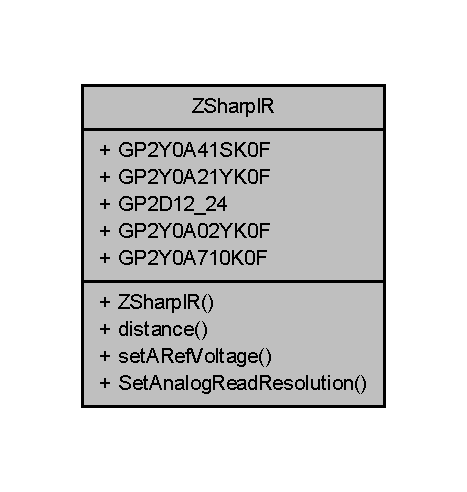
\includegraphics[width=224pt]{class_z_sharp_i_r__coll__graph}
\end{center}
\end{figure}
\subsubsection*{Public Member Functions}
\begin{DoxyCompactItemize}
\item 
\mbox{\hyperlink{class_z_sharp_i_r_a988604b3702878f8af55ba939ea3efb0}{Z\+Sharp\+IR}} (int ir\+Pin, const uint32\+\_\+t \+\_\+sensor\+Type)
\item 
int \mbox{\hyperlink{class_z_sharp_i_r_aae48083d6920e98c1b657de9e03b2254}{distance}} ()
\item 
void \mbox{\hyperlink{class_z_sharp_i_r_a20db1d8e739e9799704e78345f2858a8}{set\+A\+Ref\+Voltage}} (int refV)
\begin{DoxyCompactList}\small\item\em set\+A\+Ref\+Voltage\+:set the A\+DC reference voltage\+: (default value\+: 5000mV, set to 3300mV, typically 3.\+3 on Arduino boards) \end{DoxyCompactList}\item 
void \mbox{\hyperlink{class_z_sharp_i_r_a0121005326fb7d981fcf739730a69ac1}{Set\+Analog\+Read\+Resolution}} (int res)
\begin{DoxyCompactList}\small\item\em Set\+Analog\+Read\+Resolution\+:set the A\+DC resolution \+: (default value\+: 10, set to 12, typically 10 on Arduino boards) \end{DoxyCompactList}\end{DoxyCompactItemize}
\subsubsection*{Static Public Attributes}
\begin{DoxyCompactItemize}
\item 
static const uint32\+\_\+t \mbox{\hyperlink{class_z_sharp_i_r_a26dafed1122d774ee033e9ab10387a0e}{G\+P2\+Y0\+A41\+S\+K0F}} = 430
\item 
static const uint32\+\_\+t \mbox{\hyperlink{class_z_sharp_i_r_aa079c6041afab95db89c14a179fdfff1}{G\+P2\+Y0\+A21\+Y\+K0F}} = 1080
\item 
static const uint32\+\_\+t \mbox{\hyperlink{class_z_sharp_i_r_aa57ecb5df655ad5db0bd56e7bae59862}{G\+P2\+D12\+\_\+24}} = 1081
\item 
static const uint32\+\_\+t \mbox{\hyperlink{class_z_sharp_i_r_a588056203604897b782c2ac771cd2536}{G\+P2\+Y0\+A02\+Y\+K0F}} = 20150
\item 
static const uint32\+\_\+t \mbox{\hyperlink{class_z_sharp_i_r_a06fb0d712f9124a1d9a5183bd4e5c2b4}{G\+P2\+Y0\+A710\+K0F}} = 100500
\end{DoxyCompactItemize}


\subsubsection{Detailed Description}


Definition at line 25 of file Z\+Sharp\+I\+R.\+h.



\subsubsection{Constructor \& Destructor Documentation}
\mbox{\Hypertarget{class_z_sharp_i_r_a988604b3702878f8af55ba939ea3efb0}\label{class_z_sharp_i_r_a988604b3702878f8af55ba939ea3efb0}} 
\index{Z\+Sharp\+IR@{Z\+Sharp\+IR}!Z\+Sharp\+IR@{Z\+Sharp\+IR}}
\index{Z\+Sharp\+IR@{Z\+Sharp\+IR}!Z\+Sharp\+IR@{Z\+Sharp\+IR}}
\paragraph{\texorpdfstring{Z\+Sharp\+I\+R()}{ZSharpIR()}}
{\footnotesize\ttfamily Z\+Sharp\+I\+R\+::\+Z\+Sharp\+IR (\begin{DoxyParamCaption}\item[{int}]{ir\+Pin,  }\item[{const uint32\+\_\+t}]{\+\_\+sensor\+Type }\end{DoxyParamCaption})}



Definition at line 30 of file Z\+Sharp\+I\+R.\+cpp.



\subsubsection{Member Function Documentation}
\mbox{\Hypertarget{class_z_sharp_i_r_aae48083d6920e98c1b657de9e03b2254}\label{class_z_sharp_i_r_aae48083d6920e98c1b657de9e03b2254}} 
\index{Z\+Sharp\+IR@{Z\+Sharp\+IR}!distance@{distance}}
\index{distance@{distance}!Z\+Sharp\+IR@{Z\+Sharp\+IR}}
\paragraph{\texorpdfstring{distance()}{distance()}}
{\footnotesize\ttfamily int Z\+Sharp\+I\+R\+::distance (\begin{DoxyParamCaption}{ }\end{DoxyParamCaption})}



Definition at line 58 of file Z\+Sharp\+I\+R.\+cpp.



References G\+P2\+D12\+\_\+24, and N\+B\+\_\+\+S\+A\+M\+P\+LE.

\mbox{\Hypertarget{class_z_sharp_i_r_a0121005326fb7d981fcf739730a69ac1}\label{class_z_sharp_i_r_a0121005326fb7d981fcf739730a69ac1}} 
\index{Z\+Sharp\+IR@{Z\+Sharp\+IR}!Set\+Analog\+Read\+Resolution@{Set\+Analog\+Read\+Resolution}}
\index{Set\+Analog\+Read\+Resolution@{Set\+Analog\+Read\+Resolution}!Z\+Sharp\+IR@{Z\+Sharp\+IR}}
\paragraph{\texorpdfstring{Set\+Analog\+Read\+Resolution()}{SetAnalogReadResolution()}}
{\footnotesize\ttfamily void Z\+Sharp\+I\+R\+::\+Set\+Analog\+Read\+Resolution (\begin{DoxyParamCaption}\item[{int}]{res }\end{DoxyParamCaption})}



Set\+Analog\+Read\+Resolution\+:set the A\+DC resolution \+: (default value\+: 10, set to 12, typically 10 on Arduino boards) 



Definition at line 158 of file Z\+Sharp\+I\+R.\+cpp.

\mbox{\Hypertarget{class_z_sharp_i_r_a20db1d8e739e9799704e78345f2858a8}\label{class_z_sharp_i_r_a20db1d8e739e9799704e78345f2858a8}} 
\index{Z\+Sharp\+IR@{Z\+Sharp\+IR}!set\+A\+Ref\+Voltage@{set\+A\+Ref\+Voltage}}
\index{set\+A\+Ref\+Voltage@{set\+A\+Ref\+Voltage}!Z\+Sharp\+IR@{Z\+Sharp\+IR}}
\paragraph{\texorpdfstring{set\+A\+Ref\+Voltage()}{setARefVoltage()}}
{\footnotesize\ttfamily void Z\+Sharp\+I\+R\+::set\+A\+Ref\+Voltage (\begin{DoxyParamCaption}\item[{int}]{refV }\end{DoxyParamCaption})}



set\+A\+Ref\+Voltage\+:set the A\+DC reference voltage\+: (default value\+: 5000mV, set to 3300mV, typically 3.\+3 on Arduino boards) 



Definition at line 150 of file Z\+Sharp\+I\+R.\+cpp.



\subsubsection{Field Documentation}
\mbox{\Hypertarget{class_z_sharp_i_r_aa57ecb5df655ad5db0bd56e7bae59862}\label{class_z_sharp_i_r_aa57ecb5df655ad5db0bd56e7bae59862}} 
\index{Z\+Sharp\+IR@{Z\+Sharp\+IR}!G\+P2\+D12\+\_\+24@{G\+P2\+D12\+\_\+24}}
\index{G\+P2\+D12\+\_\+24@{G\+P2\+D12\+\_\+24}!Z\+Sharp\+IR@{Z\+Sharp\+IR}}
\paragraph{\texorpdfstring{G\+P2\+D12\+\_\+24}{GP2D12\_24}}
{\footnotesize\ttfamily const uint32\+\_\+t Z\+Sharp\+I\+R\+::\+G\+P2\+D12\+\_\+24 = 1081\hspace{0.3cm}{\ttfamily [static]}}



Definition at line 34 of file Z\+Sharp\+I\+R.\+h.



Referenced by distance().

\mbox{\Hypertarget{class_z_sharp_i_r_a588056203604897b782c2ac771cd2536}\label{class_z_sharp_i_r_a588056203604897b782c2ac771cd2536}} 
\index{Z\+Sharp\+IR@{Z\+Sharp\+IR}!G\+P2\+Y0\+A02\+Y\+K0F@{G\+P2\+Y0\+A02\+Y\+K0F}}
\index{G\+P2\+Y0\+A02\+Y\+K0F@{G\+P2\+Y0\+A02\+Y\+K0F}!Z\+Sharp\+IR@{Z\+Sharp\+IR}}
\paragraph{\texorpdfstring{G\+P2\+Y0\+A02\+Y\+K0F}{GP2Y0A02YK0F}}
{\footnotesize\ttfamily const uint32\+\_\+t Z\+Sharp\+I\+R\+::\+G\+P2\+Y0\+A02\+Y\+K0F = 20150\hspace{0.3cm}{\ttfamily [static]}}



Definition at line 35 of file Z\+Sharp\+I\+R.\+h.

\mbox{\Hypertarget{class_z_sharp_i_r_aa079c6041afab95db89c14a179fdfff1}\label{class_z_sharp_i_r_aa079c6041afab95db89c14a179fdfff1}} 
\index{Z\+Sharp\+IR@{Z\+Sharp\+IR}!G\+P2\+Y0\+A21\+Y\+K0F@{G\+P2\+Y0\+A21\+Y\+K0F}}
\index{G\+P2\+Y0\+A21\+Y\+K0F@{G\+P2\+Y0\+A21\+Y\+K0F}!Z\+Sharp\+IR@{Z\+Sharp\+IR}}
\paragraph{\texorpdfstring{G\+P2\+Y0\+A21\+Y\+K0F}{GP2Y0A21YK0F}}
{\footnotesize\ttfamily const uint32\+\_\+t Z\+Sharp\+I\+R\+::\+G\+P2\+Y0\+A21\+Y\+K0F = 1080\hspace{0.3cm}{\ttfamily [static]}}



Definition at line 33 of file Z\+Sharp\+I\+R.\+h.

\mbox{\Hypertarget{class_z_sharp_i_r_a26dafed1122d774ee033e9ab10387a0e}\label{class_z_sharp_i_r_a26dafed1122d774ee033e9ab10387a0e}} 
\index{Z\+Sharp\+IR@{Z\+Sharp\+IR}!G\+P2\+Y0\+A41\+S\+K0F@{G\+P2\+Y0\+A41\+S\+K0F}}
\index{G\+P2\+Y0\+A41\+S\+K0F@{G\+P2\+Y0\+A41\+S\+K0F}!Z\+Sharp\+IR@{Z\+Sharp\+IR}}
\paragraph{\texorpdfstring{G\+P2\+Y0\+A41\+S\+K0F}{GP2Y0A41SK0F}}
{\footnotesize\ttfamily const uint32\+\_\+t Z\+Sharp\+I\+R\+::\+G\+P2\+Y0\+A41\+S\+K0F = 430\hspace{0.3cm}{\ttfamily [static]}}



Definition at line 32 of file Z\+Sharp\+I\+R.\+h.

\mbox{\Hypertarget{class_z_sharp_i_r_a06fb0d712f9124a1d9a5183bd4e5c2b4}\label{class_z_sharp_i_r_a06fb0d712f9124a1d9a5183bd4e5c2b4}} 
\index{Z\+Sharp\+IR@{Z\+Sharp\+IR}!G\+P2\+Y0\+A710\+K0F@{G\+P2\+Y0\+A710\+K0F}}
\index{G\+P2\+Y0\+A710\+K0F@{G\+P2\+Y0\+A710\+K0F}!Z\+Sharp\+IR@{Z\+Sharp\+IR}}
\paragraph{\texorpdfstring{G\+P2\+Y0\+A710\+K0F}{GP2Y0A710K0F}}
{\footnotesize\ttfamily const uint32\+\_\+t Z\+Sharp\+I\+R\+::\+G\+P2\+Y0\+A710\+K0F = 100500\hspace{0.3cm}{\ttfamily [static]}}



Definition at line 36 of file Z\+Sharp\+I\+R.\+h.



The documentation for this class was generated from the following files\+:\begin{DoxyCompactItemize}
\item 
C\+:/\+Users/\+M43507/\+Documents/\+Arduino/libraries/\+Z\+Sharp\+I\+R/\mbox{\hyperlink{_z_sharp_i_r_8h}{Z\+Sharp\+I\+R.\+h}}\item 
C\+:/\+Users/\+M43507/\+Documents/\+Arduino/libraries/\+Z\+Sharp\+I\+R/\mbox{\hyperlink{_z_sharp_i_r_8cpp}{Z\+Sharp\+I\+R.\+cpp}}\end{DoxyCompactItemize}

\section{File Documentation}
\hypertarget{_r_e_a_d_m_e_8md}{}\subsection{C\+:/\+Users/\+M43507/\+Documents/\+Arduino/libraries/\+Z\+Sharp\+I\+R/\+R\+E\+A\+D\+ME.md File Reference}
\label{_r_e_a_d_m_e_8md}\index{C\+:/\+Users/\+M43507/\+Documents/\+Arduino/libraries/\+Z\+Sharp\+I\+R/\+R\+E\+A\+D\+M\+E.\+md@{C\+:/\+Users/\+M43507/\+Documents/\+Arduino/libraries/\+Z\+Sharp\+I\+R/\+R\+E\+A\+D\+M\+E.\+md}}

\hypertarget{_z_sharp_i_r_8cpp}{}\subsection{C\+:/\+Users/\+M43507/\+Documents/\+Arduino/libraries/\+Z\+Sharp\+I\+R/\+Z\+Sharp\+IR.cpp File Reference}
\label{_z_sharp_i_r_8cpp}\index{C\+:/\+Users/\+M43507/\+Documents/\+Arduino/libraries/\+Z\+Sharp\+I\+R/\+Z\+Sharp\+I\+R.\+cpp@{C\+:/\+Users/\+M43507/\+Documents/\+Arduino/libraries/\+Z\+Sharp\+I\+R/\+Z\+Sharp\+I\+R.\+cpp}}
{\ttfamily \#include \char`\"{}Arduino.\+h\char`\"{}}\newline
{\ttfamily \#include \char`\"{}W\+Math.\+h\char`\"{}}\newline
{\ttfamily \#include \char`\"{}Z\+Sharp\+I\+R.\+h\char`\"{}}\newline
Include dependency graph for Z\+Sharp\+I\+R.\+cpp\+:\nopagebreak
\begin{figure}[H]
\begin{center}
\leavevmode
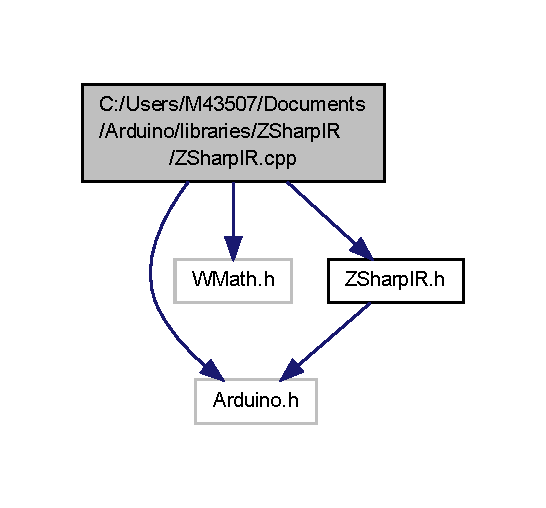
\includegraphics[width=262pt]{_z_sharp_i_r_8cpp__incl}
\end{center}
\end{figure}

\hypertarget{_z_sharp_i_r_8h}{}\subsection{C\+:/\+Users/\+M43507/\+Documents/\+Arduino/libraries/\+Z\+Sharp\+I\+R/\+Z\+Sharp\+IR.h File Reference}
\label{_z_sharp_i_r_8h}\index{C\+:/\+Users/\+M43507/\+Documents/\+Arduino/libraries/\+Z\+Sharp\+I\+R/\+Z\+Sharp\+I\+R.\+h@{C\+:/\+Users/\+M43507/\+Documents/\+Arduino/libraries/\+Z\+Sharp\+I\+R/\+Z\+Sharp\+I\+R.\+h}}
{\ttfamily \#include \char`\"{}Arduino.\+h\char`\"{}}\newline
Include dependency graph for Z\+Sharp\+I\+R.\+h\+:\nopagebreak
\begin{figure}[H]
\begin{center}
\leavevmode
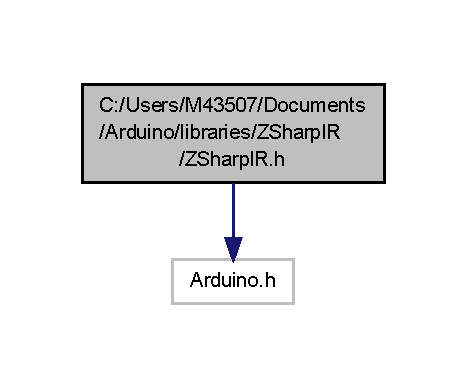
\includegraphics[width=224pt]{_z_sharp_i_r_8h__incl}
\end{center}
\end{figure}
This graph shows which files directly or indirectly include this file\+:\nopagebreak
\begin{figure}[H]
\begin{center}
\leavevmode
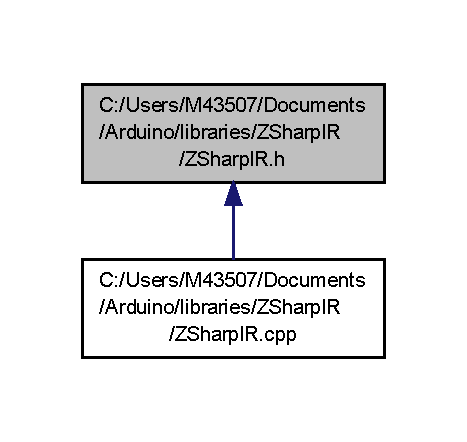
\includegraphics[width=224pt]{_z_sharp_i_r_8h__dep__incl}
\end{center}
\end{figure}
\subsubsection*{Data Structures}
\begin{DoxyCompactItemize}
\item 
class \mbox{\hyperlink{class_z_sharp_i_r}{Z\+Sharp\+IR}}
\end{DoxyCompactItemize}
\subsubsection*{Macros}
\begin{DoxyCompactItemize}
\item 
\#define \mbox{\hyperlink{_z_sharp_i_r_8h_a2b27a5d5abd22a410012f5a29d397699}{N\+B\+\_\+\+S\+A\+M\+P\+LE}}~10
\end{DoxyCompactItemize}


\subsubsection{Macro Definition Documentation}
\mbox{\Hypertarget{_z_sharp_i_r_8h_a2b27a5d5abd22a410012f5a29d397699}\label{_z_sharp_i_r_8h_a2b27a5d5abd22a410012f5a29d397699}} 
\index{Z\+Sharp\+I\+R.\+h@{Z\+Sharp\+I\+R.\+h}!N\+B\+\_\+\+S\+A\+M\+P\+LE@{N\+B\+\_\+\+S\+A\+M\+P\+LE}}
\index{N\+B\+\_\+\+S\+A\+M\+P\+LE@{N\+B\+\_\+\+S\+A\+M\+P\+LE}!Z\+Sharp\+I\+R.\+h@{Z\+Sharp\+I\+R.\+h}}
\paragraph{\texorpdfstring{N\+B\+\_\+\+S\+A\+M\+P\+LE}{NB\_SAMPLE}}
{\footnotesize\ttfamily \#define N\+B\+\_\+\+S\+A\+M\+P\+LE~10}



Definition at line 17 of file Z\+Sharp\+I\+R.\+h.



Referenced by Z\+Sharp\+I\+R\+::distance().


%--- End generated contents ---

% Index
\newpage
\phantomsection
\clearemptydoublepage
\addcontentsline{toc}{section}{Index}
\printindex

\end{document}
